\chapter{Conclusion and outlook}
\label{cha:conclusion}

This chapter summarises the achievements of this thesis and lists features which might be implemented in the future.

\section{Conclusion}
\label{sec:conclusion}

This thesis provides a software architecture and a description of its implementation that allows to develop, simulate, play and analyse any round-based business game in a browser. This system is called Business Game Engine (BGE) while its description mechanism for round-based business games is called Business Game Description (BGD).

A first literature review showed how similar efforts have been carried out in Japan with the work on BMDL, BMDS and YBG between 1997 and 2007. 

Then, a framework for general n-person round-based games as a 7-tuple of turn-based inputs, fixed  parameters, outputs, initial game state, state transition functions, score function and a stop condition is introduced. This framework provides a clear definition of round-based games allowing to mathematically describe each member of that class.

In chapter \ref{cha:architecture} the design of the proposed architecture is described in detail as one major contribution of this thesis. In contrast to the work in Japan an object model is proposed, with which a round-based game can be described using any general purpose object-oriented programming language instead of defining a new programming language. This drastically simplifies the implementation of such a system since we used an open-source Javascript parser and also allows to make use of existing libraries. It maintains at the same time a very high flexibility since game developers can use any feature of the programming language that is being used. 

The second major contribution is the implementation of the proposed architecture. A prototype is running on \textit{http://games.fkmt.de}. It uses the most recent (web)technologies such as server-side Javascript, NoSQL and WebSockets. The consistent use of Javascript allows to smoothly shift tasks between server and client and to natively use JSON objects all around the architecture. Most of the load has been shifted to the clients which allows a secure execution of untrusted game code within the Browser's sandbox as well as a deployment with very limited physical resources. The general use of JSON objects in combination with WebSockets leads to a very efficient communication and synchronization between server and client, enormously facilitating the implementation of such a complex system. Finally, the use of a modern NoSQL database allowing to save JSON objects directly avoids the need for an expensive object-relational mapping (ORM).

\section{Future work}
\label{sec:futurework}

Future work might be done on the definition and implementation of BGD (roles, table-based output) as well as on the entrance hall module and the analysis environment.

\subsection{Roles}
\label{sub:conclusion:roles}

BGD could be extended with a role functionality. A business game could then have several roles and one of these roles would be assigned to each player. The inputs, outputs, parameters, state-transition-functions and score function could then be made dependent on the player's role. The beergame for example knows the roles retailer, wholesaler, distributor and factory, eventhough it can also be implemented without roles (see appendix).

\subsection{Advanced entrance hall}
\label{sub:conclusion:entrance}

The entrance hall module could be extended functionally so that the entrance hall becomes a separate html page. This page consists of $n$ player slots and a start button, where $n$ is the maximal number of players that can participate in the game. Each player who joins the game gets assigned to one player slot. The game creator, who is the first person joining the game, can additionally assign empty slots to virtual opponents. He can start the game after the number of assigned slots lies between the minimal and maximal number of players of the business game.

\subsection{Advanced analysis environment}
\label{sub:conclusion:analysis}

This prototype implementation provides a download functionality for all prior played game sessions of a specific BG as JSON file. Data analysts who want to filter this data for specific criteria either have to query MongoDB directly (if they have been granted access to it) or need to parse the JSON data and implement their own analysis environment around that. This can be done relatively easy since JSON utilities exist for all recent programming languages. 

Nevertheless future implementations might implement an advanced analysis environment directly. This environment might query the database for global or local game criteria. Global criteria might be \textit{all games},  \textit{all games without player abort}, \textit{all games with questionnaire data} and so on. Local criteria might be realised in form of query rules as shown in figure \ref{fig:analysis}.

\begin{figure}
	\centering
	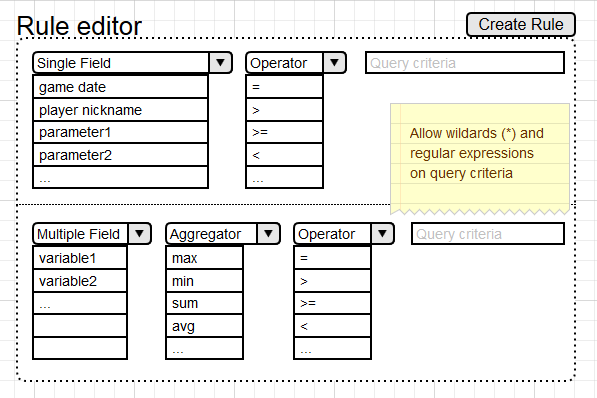
\includegraphics[scale=0.65]{figures/analysis.png}
	\caption{Example UI for a local query criteria rule generator}
	\label{fig:analysis}
\end{figure}

The result of this query, using global and/or local game criteria, might again be a JSON file. An advanced analysis environment might also implement a relational mapping of JSON game data so that the query result can be displayed in tables in an online view or provided as table based csv-export for example for spreadsheet programs. If implemented in a generic way, such a mapping might be the basis of an ORM so that BGE can be used together with relational databases as well.

\subsection{Tabular output}
\label{sub:conclusion:table}

In the current implementation, variable outcomes are visualised with charts, giving all players complete information about that variable. A chart furthermore only visualises one variable at a time. Rendering output as tables might be used to address both issues, enabling incomplete information as well as displaying related things in one place. 

Listing \ref{lst:table} shows how table-based output could be realised in the BGD game code using the example of the order input variable in the beergame which should have incomplete information.

\begin{lstlisting}[language=Javascript, caption=BGD table extension: orders in the beergame, label=lst:table,float,floatplacement=H]
// Custom table showing each player of the beergame only the orders 
// he is allowed to see (incomplete information)
function orderTable(playerIndex) {
    var cr = game.getCurrentRound();
    var table = {};
    table.header = 'Order table in round' + (cr+1);
    table.columns = [];
    // First row of the table. Will be printed in bold by default.
    table.columns.push("Round number", "Orders from client");
    // Go through all rounds and add orders from player's client
    var orders;
    var orderDelay = game.getParameter("orderReceivingDelay");
    for (var roundIndex = 0; roundIndex <= cr; roundIndex++) {
        var orderRoundNumber = roundIndex - orderDelay;
        if (playerIndex === 0) { // retailer
            orders = game.get("customerDemand", orderRoundNumber);
        } else { // wholesaler, distributor, factory
            orders = game.get("order", orderRoundNumber, playerIndex-1);
        }
        table.columns.push(roundIndex + 1, orders);
    }
    return table; // Each custom-defined table must return such an object
}
// Register tables in the architecture
game.registerTables([orderTable, otherCustomTable, preDefinedTable, ...]);

/*
There might be other pre-defined tables such as 
roundResultTable (all players' variable results of the last round)
or playerResultTable (all variable results of this player for all rounds).
These tables could also be registered with the game.registerTables() method.
*/
\end{lstlisting}
